% Options for packages loaded elsewhere
\PassOptionsToPackage{unicode}{hyperref}
\PassOptionsToPackage{hyphens}{url}
%
\documentclass[
  11pt,
  ignorenonframetext,
]{beamer}
\usepackage{pgfpages}
\setbeamertemplate{caption}[numbered]
\setbeamertemplate{caption label separator}{: }
\setbeamercolor{caption name}{fg=normal text.fg}
\beamertemplatenavigationsymbolsempty
% Prevent slide breaks in the middle of a paragraph
\widowpenalties 1 10000
\raggedbottom
\setbeamertemplate{part page}{
  \centering
  \begin{beamercolorbox}[sep=16pt,center]{part title}
    \usebeamerfont{part title}\insertpart\par
  \end{beamercolorbox}
}
\setbeamertemplate{section page}{
  \centering
  \begin{beamercolorbox}[sep=12pt,center]{part title}
    \usebeamerfont{section title}\insertsection\par
  \end{beamercolorbox}
}
\setbeamertemplate{subsection page}{
  \centering
  \begin{beamercolorbox}[sep=8pt,center]{part title}
    \usebeamerfont{subsection title}\insertsubsection\par
  \end{beamercolorbox}
}
\AtBeginPart{
  \frame{\partpage}
}
\AtBeginSection{
  \ifbibliography
  \else
    \frame{\sectionpage}
  \fi
}
\AtBeginSubsection{
  \frame{\subsectionpage}
}
\usepackage{amsmath,amssymb}
\usepackage{iftex}
\ifPDFTeX
  \usepackage[T1]{fontenc}
  \usepackage[utf8]{inputenc}
  \usepackage{textcomp} % provide euro and other symbols
\else % if luatex or xetex
  \usepackage{unicode-math} % this also loads fontspec
  \defaultfontfeatures{Scale=MatchLowercase}
  \defaultfontfeatures[\rmfamily]{Ligatures=TeX,Scale=1}
\fi
\usepackage{lmodern}
\usetheme[]{metropolis}
\ifPDFTeX\else
  % xetex/luatex font selection
\fi
% Use upquote if available, for straight quotes in verbatim environments
\IfFileExists{upquote.sty}{\usepackage{upquote}}{}
\IfFileExists{microtype.sty}{% use microtype if available
  \usepackage[]{microtype}
  \UseMicrotypeSet[protrusion]{basicmath} % disable protrusion for tt fonts
}{}
\makeatletter
\@ifundefined{KOMAClassName}{% if non-KOMA class
  \IfFileExists{parskip.sty}{%
    \usepackage{parskip}
  }{% else
    \setlength{\parindent}{0pt}
    \setlength{\parskip}{6pt plus 2pt minus 1pt}}
}{% if KOMA class
  \KOMAoptions{parskip=half}}
\makeatother
\usepackage{xcolor}
\newif\ifbibliography
\usepackage{color}
\usepackage{fancyvrb}
\newcommand{\VerbBar}{|}
\newcommand{\VERB}{\Verb[commandchars=\\\{\}]}
\DefineVerbatimEnvironment{Highlighting}{Verbatim}{commandchars=\\\{\}}
% Add ',fontsize=\small' for more characters per line
\newenvironment{Shaded}{}{}
\newcommand{\AlertTok}[1]{\textcolor[rgb]{1.00,0.00,0.00}{\textbf{#1}}}
\newcommand{\AnnotationTok}[1]{\textcolor[rgb]{0.38,0.63,0.69}{\textbf{\textit{#1}}}}
\newcommand{\AttributeTok}[1]{\textcolor[rgb]{0.49,0.56,0.16}{#1}}
\newcommand{\BaseNTok}[1]{\textcolor[rgb]{0.25,0.63,0.44}{#1}}
\newcommand{\BuiltInTok}[1]{\textcolor[rgb]{0.00,0.50,0.00}{#1}}
\newcommand{\CharTok}[1]{\textcolor[rgb]{0.25,0.44,0.63}{#1}}
\newcommand{\CommentTok}[1]{\textcolor[rgb]{0.38,0.63,0.69}{\textit{#1}}}
\newcommand{\CommentVarTok}[1]{\textcolor[rgb]{0.38,0.63,0.69}{\textbf{\textit{#1}}}}
\newcommand{\ConstantTok}[1]{\textcolor[rgb]{0.53,0.00,0.00}{#1}}
\newcommand{\ControlFlowTok}[1]{\textcolor[rgb]{0.00,0.44,0.13}{\textbf{#1}}}
\newcommand{\DataTypeTok}[1]{\textcolor[rgb]{0.56,0.13,0.00}{#1}}
\newcommand{\DecValTok}[1]{\textcolor[rgb]{0.25,0.63,0.44}{#1}}
\newcommand{\DocumentationTok}[1]{\textcolor[rgb]{0.73,0.13,0.13}{\textit{#1}}}
\newcommand{\ErrorTok}[1]{\textcolor[rgb]{1.00,0.00,0.00}{\textbf{#1}}}
\newcommand{\ExtensionTok}[1]{#1}
\newcommand{\FloatTok}[1]{\textcolor[rgb]{0.25,0.63,0.44}{#1}}
\newcommand{\FunctionTok}[1]{\textcolor[rgb]{0.02,0.16,0.49}{#1}}
\newcommand{\ImportTok}[1]{\textcolor[rgb]{0.00,0.50,0.00}{\textbf{#1}}}
\newcommand{\InformationTok}[1]{\textcolor[rgb]{0.38,0.63,0.69}{\textbf{\textit{#1}}}}
\newcommand{\KeywordTok}[1]{\textcolor[rgb]{0.00,0.44,0.13}{\textbf{#1}}}
\newcommand{\NormalTok}[1]{#1}
\newcommand{\OperatorTok}[1]{\textcolor[rgb]{0.40,0.40,0.40}{#1}}
\newcommand{\OtherTok}[1]{\textcolor[rgb]{0.00,0.44,0.13}{#1}}
\newcommand{\PreprocessorTok}[1]{\textcolor[rgb]{0.74,0.48,0.00}{#1}}
\newcommand{\RegionMarkerTok}[1]{#1}
\newcommand{\SpecialCharTok}[1]{\textcolor[rgb]{0.25,0.44,0.63}{#1}}
\newcommand{\SpecialStringTok}[1]{\textcolor[rgb]{0.73,0.40,0.53}{#1}}
\newcommand{\StringTok}[1]{\textcolor[rgb]{0.25,0.44,0.63}{#1}}
\newcommand{\VariableTok}[1]{\textcolor[rgb]{0.10,0.09,0.49}{#1}}
\newcommand{\VerbatimStringTok}[1]{\textcolor[rgb]{0.25,0.44,0.63}{#1}}
\newcommand{\WarningTok}[1]{\textcolor[rgb]{0.38,0.63,0.69}{\textbf{\textit{#1}}}}
\usepackage{longtable,booktabs,array}
\usepackage{calc} % for calculating minipage widths
\usepackage{caption}
% Make caption package work with longtable
\makeatletter
\def\fnum@table{\tablename~\thetable}
\makeatother
\usepackage{graphicx}
\makeatletter
\def\maxwidth{\ifdim\Gin@nat@width>\linewidth\linewidth\else\Gin@nat@width\fi}
\def\maxheight{\ifdim\Gin@nat@height>\textheight\textheight\else\Gin@nat@height\fi}
\makeatother
% Scale images if necessary, so that they will not overflow the page
% margins by default, and it is still possible to overwrite the defaults
% using explicit options in \includegraphics[width, height, ...]{}
\setkeys{Gin}{width=\maxwidth,height=\maxheight,keepaspectratio}
% Set default figure placement to htbp
\makeatletter
\def\fps@figure{htbp}
\makeatother
\setlength{\emergencystretch}{3em} % prevent overfull lines
\providecommand{\tightlist}{%
  \setlength{\itemsep}{0pt}\setlength{\parskip}{0pt}}
\setcounter{secnumdepth}{-\maxdimen} % remove section numbering
\ifLuaTeX
  \usepackage{selnolig}  % disable illegal ligatures
\fi
\IfFileExists{bookmark.sty}{\usepackage{bookmark}}{\usepackage{hyperref}}
\IfFileExists{xurl.sty}{\usepackage{xurl}}{} % add URL line breaks if available
\urlstyle{same}
\hypersetup{
  pdftitle={Análisis de la asociación espacial},
  pdfauthor={Gerardo Martín},
  hidelinks,
  pdfcreator={LaTeX via pandoc}}

\title{Análisis de la asociación espacial}
\subtitle{Correlación entre variables espaciales}
\author{Gerardo Martín}
\date{2022-06-29}

\begin{document}
\frame{\titlepage}

\begin{frame}{Las variables espaciales}
\protect\hypertarget{las-variables-espaciales}{}
Además de valores de varibles, tenemos ubicación, p.~ej.

\begin{longtable}[]{@{}rrrrr@{}}
\caption{Primeras seis filas de una conjunto de variables raster
tabuladas. Las coordenadas corresponden al centro de cada
píxel.}\tabularnewline
\toprule\noalign{}
x & y & Var-1 & Var-2 & Var-3 \\
\midrule\noalign{}
\endfirsthead
\toprule\noalign{}
x & y & Var-1 & Var-2 & Var-3 \\
\midrule\noalign{}
\endhead
-104.8380 & 29.93903 & 186 & 92 & 173 \\
-104.6714 & 29.93903 & 190 & 96 & 178 \\
-104.5047 & 29.93903 & 188 & 95 & 179 \\
-104.3380 & 29.93903 & 166 & 79 & 165 \\
-104.1714 & 29.93903 & 171 & 83 & 170 \\
-104.0047 & 29.93903 & 176 & 87 & 174 \\
\bottomrule\noalign{}
\end{longtable}
\end{frame}

\begin{frame}{Las variables espaciales}
\protect\hypertarget{las-variables-espaciales-1}{}
\begin{figure}

{\centering 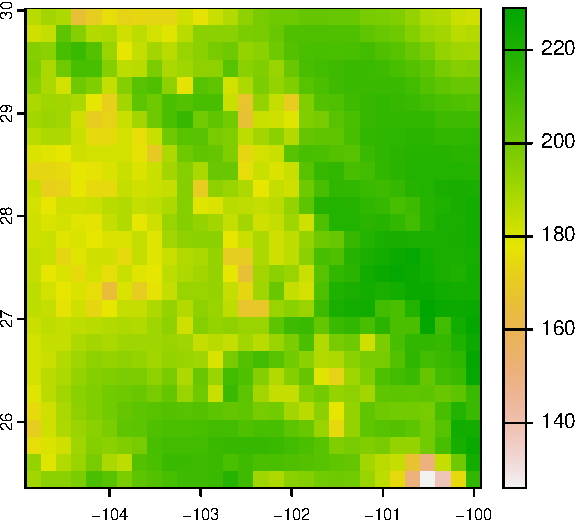
\includegraphics{Correlacion-espacial_files/figure-beamer/unnamed-chunk-2-1} 

}

\caption{Gráfico de la variable 1.}\label{fig:unnamed-chunk-2}
\end{figure}
\end{frame}

\begin{frame}{Las variables espaciales}
\protect\hypertarget{las-variables-espaciales-2}{}
\begin{center}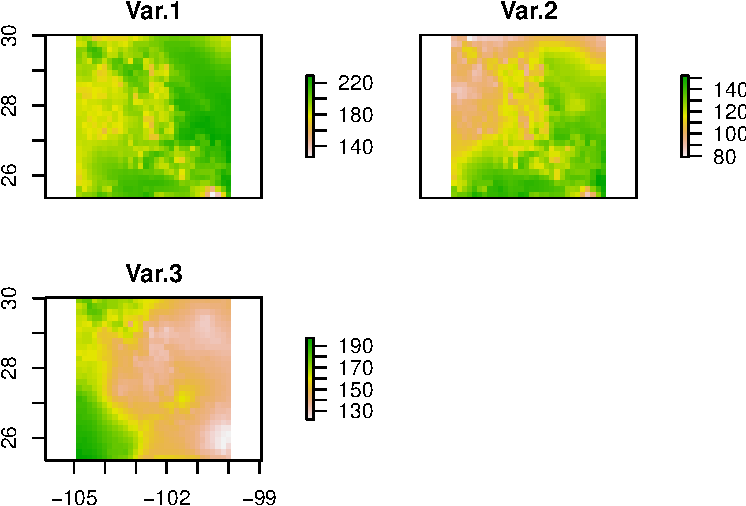
\includegraphics{Correlacion-espacial_files/figure-beamer/unnamed-chunk-3-1} \end{center}
\end{frame}

\begin{frame}{Correlación entre variables espaciales}
\protect\hypertarget{correlaciuxf3n-entre-variables-espaciales}{}
Comparando las paletas de color, no nos es del todo posible detectar
correlaciones.

Necesitamos:

\begin{enumerate}
\item
  Gráfico de dispersión
\item
  Coeficiente de correlación
\end{enumerate}
\end{frame}

\begin{frame}[fragile]{Correlación entre variables espaciales}
\protect\hypertarget{correlaciuxf3n-entre-variables-espaciales-1}{}
Paquete \texttt{raster} contiene métodos para hacer el cálculo entre
pares de capas

Función \texttt{pairs} hace todo en automático, uso

\begin{Shaded}
\begin{Highlighting}[]
\FunctionTok{pairs}\NormalTok{(raster)}
\end{Highlighting}
\end{Shaded}
\end{frame}

\begin{frame}[fragile]{Uso de \texttt{pairs}}
\protect\hypertarget{uso-de-pairs}{}
\begin{itemize}
\item
  Único argumento necesario, nombre de objeto tipo \texttt{raster},
  \texttt{stack} ó \texttt{brick}
\item
  En ejemplo anterior, el nombre del objeto es \texttt{raster},
  necesitamos otro nombre
\end{itemize}

\begin{Shaded}
\begin{Highlighting}[]
\CommentTok{\# para una sola capa}
\NormalTok{r }\OtherTok{\textless{}{-}} \FunctionTok{rast}\NormalTok{(}\StringTok{"../Datos{-}ejemplos/Var{-}1.tif"}\NormalTok{) }
\CommentTok{\#Para varias capas alineadas}
\NormalTok{r }\OtherTok{\textless{}{-}} \FunctionTok{rast}\NormalTok{(}\FunctionTok{list.files}\NormalTok{(}\StringTok{"../Datos{-}ejemplos/"}\NormalTok{, }
                      \StringTok{"tif"}\NormalTok{, }\AttributeTok{full.names =}\NormalTok{ T))}
\end{Highlighting}
\end{Shaded}
\end{frame}

\begin{frame}[fragile]{Uso de pairs}
\protect\hypertarget{uso-de-pairs-1}{}
\begin{Shaded}
\begin{Highlighting}[]
\FunctionTok{pairs}\NormalTok{(r)}
\end{Highlighting}
\end{Shaded}

\begin{center}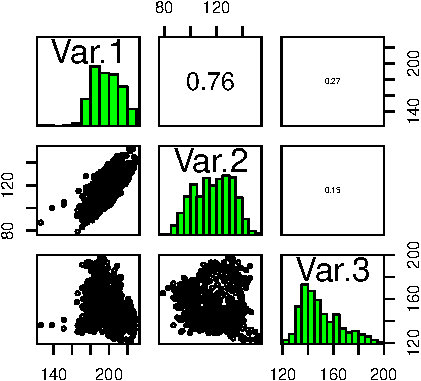
\includegraphics{Correlacion-espacial_files/figure-beamer/unnamed-chunk-6-1} \end{center}
\end{frame}

\begin{frame}{Interpretación de gráfico de pares}
\protect\hypertarget{interpretaciuxf3n-de-gruxe1fico-de-pares}{}
\begin{itemize}
\item
  Diagonal principal \(\rightarrow\) Histograma de variable individual
\item
  Triángulo inferior \(\rightarrow\) Gráfico de dispersión
\item
  Triángulo superior \(\rightarrow\) Coeficiente de correlación estimado
  (ver cálculo \href{Correlacion.pdf}{aquí})
\end{itemize}
\end{frame}

\begin{frame}{Correlación entre puntos y raster}
\protect\hypertarget{correlaciuxf3n-entre-puntos-y-raster}{}
\begin{itemize}
\tightlist
\item
  Cuando tenemos mediciones colectadas, podríamos tener sólo coordenadas
  de los puntos de muestreo
\end{itemize}

\begin{longtable}[]{@{}lrrr@{}}
\caption{Primeras seis filas de una base de datos de mediciones
colectadas en campo.}\tabularnewline
\toprule\noalign{}
& x & y & mediciones \\
\midrule\noalign{}
\endfirsthead
\toprule\noalign{}
& x & y & mediciones \\
\midrule\noalign{}
\endhead
73 & -102.7928 & 29.57881 & 49.62024 \\
459 & -103.6011 & 27.38053 & 41.14992 \\
813 & -104.5670 & 25.53772 & 137.04156 \\
49 & -101.8276 & 29.87109 & 51.70786 \\
476 & -100.5730 & 27.40428 & 103.70981 \\
144 & -101.0474 & 29.20245 & 75.43274 \\
\bottomrule\noalign{}
\end{longtable}
\end{frame}

\begin{frame}{Correlación entre puntos y raster}
\protect\hypertarget{correlaciuxf3n-entre-puntos-y-raster-1}{}
Necesitamos medir con qué proceso ambiental (representado con una capa
raster) nuestros datos están asociados

\begin{itemize}
\item
  Tenemos 3 capas:

  \begin{itemize}
  \tightlist
  \item
    Var.1, Var.2, Var.3
  \end{itemize}
\item
  Para encontrar asociación, necesitamos:

  \begin{enumerate}
  \item
    Graficar valores de variable colectada sobre capas raster
  \item
    Extraer valores en localidades de muestreo de capas raster
  \item
    Hacer prueba de correlación entre las 3 capas raster y mediciones
  \end{enumerate}
\end{itemize}
\end{frame}

\begin{frame}{Gráfico de valores colectados 1}
\protect\hypertarget{gruxe1fico-de-valores-colectados-1}{}
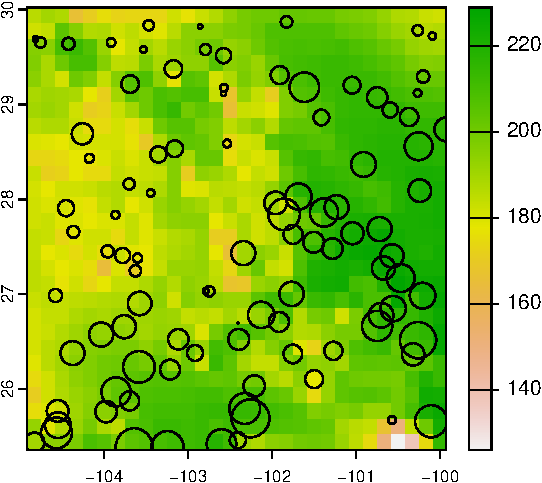
\includegraphics{Correlacion-espacial_files/figure-beamer/unnamed-chunk-8-1.pdf}
\end{frame}

\begin{frame}[fragile]{Gráfico de valores colectados 2}
\protect\hypertarget{gruxe1fico-de-valores-colectados-2}{}
\begin{Shaded}
\begin{Highlighting}[]
\FunctionTok{plot}\NormalTok{(r[[}\DecValTok{2}\NormalTok{]])}
\FunctionTok{points}\NormalTok{(puntos[, }\FunctionTok{c}\NormalTok{(}\StringTok{"x"}\NormalTok{, }\StringTok{"y"}\NormalTok{)], }\AttributeTok{cex =}\NormalTok{ puntos}\SpecialCharTok{$}\NormalTok{mediciones}\SpecialCharTok{/}\DecValTok{50}\NormalTok{)}
\end{Highlighting}
\end{Shaded}

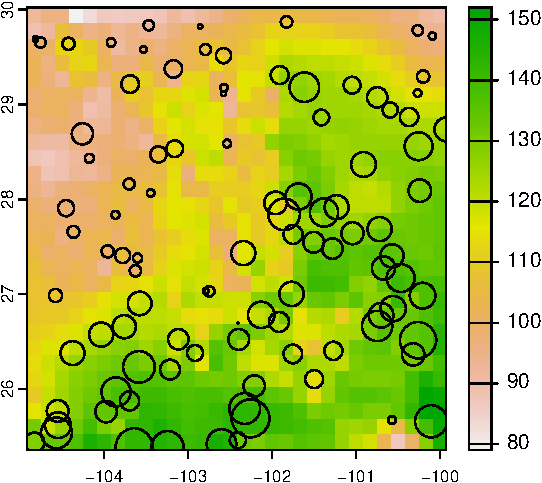
\includegraphics{Correlacion-espacial_files/figure-beamer/unnamed-chunk-9-1.pdf}
\end{frame}

\begin{frame}{Gráfico de valores colectados 3}
\protect\hypertarget{gruxe1fico-de-valores-colectados-3}{}
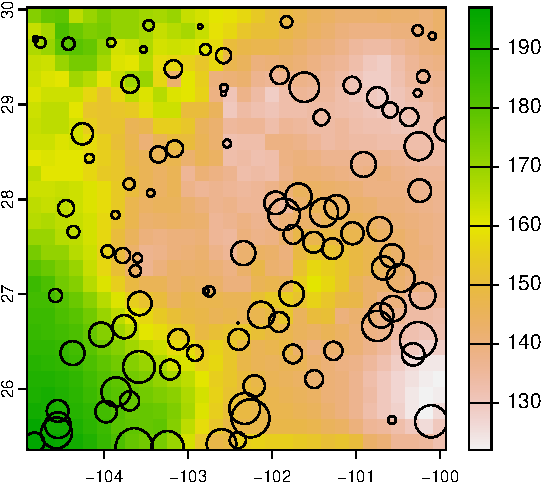
\includegraphics{Correlacion-espacial_files/figure-beamer/unnamed-chunk-10-1.pdf}
\end{frame}

\begin{frame}[fragile]{Extraer valores de capa raster}
\protect\hypertarget{extraer-valores-de-capa-raster}{}
Función \texttt{extract}, dos argumentos:

\begin{enumerate}
\item
  Capa(s) raster de dónde extraer valores
\item
  Conjunto de coordenadas para extraer valores
\end{enumerate}

\begin{Shaded}
\begin{Highlighting}[]
\NormalTok{valores.capas }\OtherTok{\textless{}{-}} \FunctionTok{extract}\NormalTok{(r, puntos[, }\FunctionTok{c}\NormalTok{(}\StringTok{"x"}\NormalTok{, }\StringTok{"y"}\NormalTok{)])}
\NormalTok{puntos }\OtherTok{\textless{}{-}} \FunctionTok{data.frame}\NormalTok{(puntos, valores.capas)}
\end{Highlighting}
\end{Shaded}

(El objeto puntos fue generado anteriormente, pueden ver detalles de
simulación en código fuente)
\end{frame}

\begin{frame}{Valores extraídos de capa raster}
\protect\hypertarget{valores-extrauxeddos-de-capa-raster}{}
\begin{longtable}[]{@{}lrrrrrrr@{}}
\toprule\noalign{}
& x & y & mediciones & ID & Var.1 & Var.2 & Var.3 \\
\midrule\noalign{}
\endhead
73 & -102.7928 & 29.57881 & 49.62024 & 1 & 199 & 106 & 161 \\
459 & -103.6011 & 27.38053 & 41.14992 & 2 & 179 & 105 & 143 \\
813 & -104.5670 & 25.53772 & 137.04156 & 3 & 187 & 126 & 193 \\
49 & -101.8276 & 29.87109 & 51.70786 & 4 & 203 & 105 & 149 \\
476 & -100.5730 & 27.40428 & 103.70981 & 5 & 224 & 135 & 143 \\
144 & -101.0474 & 29.20245 & 75.43274 & 6 & 213 & 121 & 131 \\
255 & -102.5358 & 28.58792 & 35.05952 & 7 & 174 & 101 & 132 \\
201 & -101.4132 & 28.86275 & 69.94669 & 8 & 209 & 125 & 134 \\
646 & -102.3974 & 26.52351 & 92.91473 & 9 & 211 & 134 & 153 \\
824 & -102.6020 & 25.42059 & 131.78474 & 10 & 218 & 147 & 148 \\
\bottomrule\noalign{}
\end{longtable}
\end{frame}

\begin{frame}{Gráficos de dispersión 1}
\protect\hypertarget{gruxe1ficos-de-dispersiuxf3n-1}{}
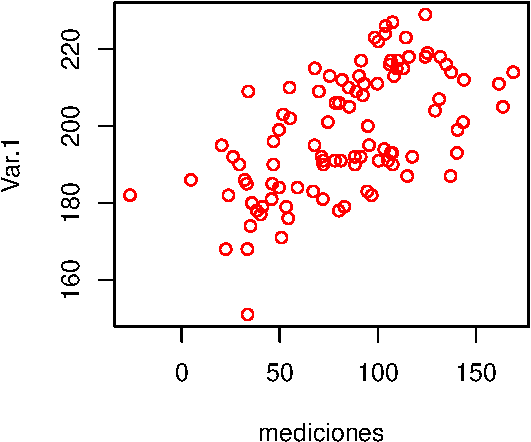
\includegraphics{Correlacion-espacial_files/figure-beamer/unnamed-chunk-13-1.pdf}
\end{frame}

\begin{frame}{Gráficos de dispersión 2}
\protect\hypertarget{gruxe1ficos-de-dispersiuxf3n-2}{}
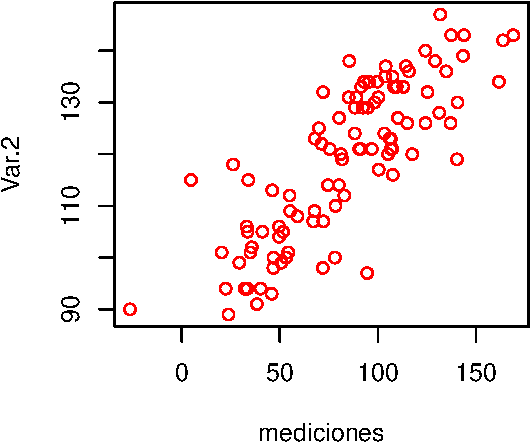
\includegraphics{Correlacion-espacial_files/figure-beamer/unnamed-chunk-14-1.pdf}
\end{frame}

\begin{frame}{Gráficos de dispersión 3}
\protect\hypertarget{gruxe1ficos-de-dispersiuxf3n-3}{}
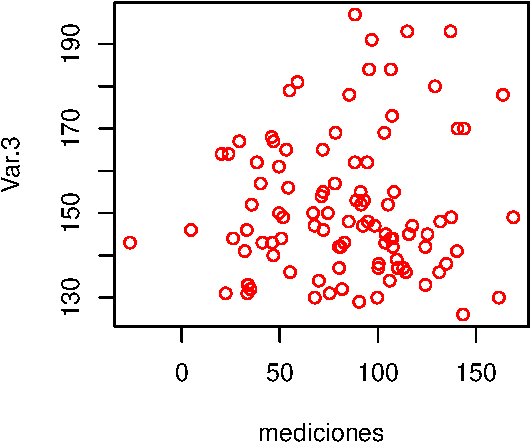
\includegraphics{Correlacion-espacial_files/figure-beamer/unnamed-chunk-15-1.pdf}
\end{frame}

\begin{frame}[fragile]{Coeficientes de correlación}
\protect\hypertarget{coeficientes-de-correlaciuxf3n}{}
\begin{Shaded}
\begin{Highlighting}[]
\FunctionTok{cor}\NormalTok{(puntos[, }\FunctionTok{c}\NormalTok{(}\StringTok{"mediciones"}\NormalTok{, }\StringTok{"Var.1"}\NormalTok{, }\StringTok{"Var.2"}\NormalTok{, }\StringTok{"Var.3"}\NormalTok{)])}
\end{Highlighting}
\end{Shaded}

\begin{verbatim}
##            mediciones      Var.1      Var.2       Var.3
## mediciones 1.00000000  0.5845601  0.8107585  0.06998098
## Var.1      0.58456009  1.0000000  0.7522413 -0.21898861
## Var.2      0.81075853  0.7522413  1.0000000 -0.01619570
## Var.3      0.06998098 -0.2189886 -0.0161957  1.00000000
\end{verbatim}
\end{frame}

\begin{frame}[fragile]{Conclusión}
\protect\hypertarget{conclusiuxf3n}{}
En ausencia de mayor información

\begin{itemize}
\tightlist
\item
  Mediciones están asociadas espacialmente con \texttt{Var.2}
\end{itemize}
\end{frame}

\end{document}
